\section{Introduction}
\label{sec:introduction}

The discovery of a Higgs ($\PHiggs$) boson by the ATLAS and CMS experiments at the LHC~\cite{Higgs-Discovery_CMS,Higgs-Discovery_ATLAS}
represents a major step towards our understanding of electroweak symmetry breaking (EWSB) 
and of the mechanism that generates the masses of quarks and leptons, the particles that constitute the ``ordinary'' matter in our universe.
In a combined analysis of the data recorded by ATLAS and CMS, 
the mass of the $\PHiggs$ boson has been measured to be $125.09 \pm 0.24$~\GeV~\cite{HIG-14-042}.
The Standard Model (SM) of particle physics makes precise predictions for all properties of the $\PHiggs$ boson, given its mass.
So far, all measured properties of the discovered particle are consistent with the expectation for a SM $\PHiggs$ boson within the uncertainties of these measurements~\cite{HIG-15-002}.
In particular, the rate for its decay into a pair of $\Pgt$ leptons has been measured with an uncertainty of $20$--$30\%$
and found to be compatible with the SM expectation~\cite{HIG-13-004,Aad:2015vsa,HIG-15-002,HIG-16-043,ATLAS:2018lur}.

Pairs of $\PHiggs$ bosons ($\PHiggs\PHiggs$) may be produced by two different mechanisms at the LHC,
referred to as ``resonant'' and ``non-resonant'' production.

Within the SM, $\PHiggs\PHiggs$ production proceeds solely via non-resonant production.
The leading order (LO) Feynman diagrams for SM $\PHiggs\PHiggs$ production are shown in Fig.~\ref{fig:FeynmanDiagrams_smHH}.
The cross section for $\PHiggs\PHiggs$ production is small, amounting to about $\sigma = 34$~fb in proton-proton collisions at $\sqrt{s}=13$~\TeV center-of-mass energy,
due to the destructive interference of the two diagrams.
The ``triangle'' diagram shown on the left depends on the trilinear self-coupling, $\lambda_{\PHiggs\PHiggs\PHiggs}$, of the $\PHiggs$ boson, 
while the ``box'' diagram shown on the right does not.
Deviations of $\lambda_{\PHiggs\PHiggs\PHiggs}$ from its SM value of $\lambda_{\textrm{SM}}=1$, referred to as anomalous $\PHiggs$ boson self-couplings,
alter the interference between the two diagrams, 
resulting in a change in the $\PHiggs\PHiggs$ production cross section and a change in the distribution of the mass, $m_{\PHiggs\PHiggs}$, of the $\PHiggs$ boson pair.
The shape of the distribution in $m_{\PHiggs\PHiggs}$ thus provides a handle to determine $\lambda_{\PHiggs\PHiggs\PHiggs}$,
complementary to measuring the $\PHiggs\PHiggs$ production cross section.
Various scenarios beyond the SM feature anomalous $\PHiggs$ boson self-couplings,
for example two-Higgs-doublet models~\cite{Branco:2011iw}, such as the minimal supersymmetric extension of the SM (MSSM)~\cite{Gunion:1989we},
and models with composite $\PHiggs$ bosons~\cite{Grober:2010yv,Contino:2012xk}.
The prospects for improving the sensitivity to determine $\lambda_{\PHiggs\PHiggs\PHiggs}$ by utilising information on the mass of the $\PHiggs$ boson pair
have been studied in events in which the $\PHiggs$ boson pair decays via $\PHiggs\PHiggs \to \PW^{+}\PW^{-}\PW^{+}\PW^{-}$, with subsequent decay of the $\PW$ bosons to electrons, muons, or jets,
in Refs.~\cite{Baur:2002rb,Baur:2002qd}.
In case of non-resonant production the information that can be extracted from the distribution in $m_{\PHiggs\PHiggs}$ is limited, however,
first because the distribution in $m_{\PHiggs\PHiggs}$ is rather broad and changes only moderately with $\lambda_{\PHiggs\PHiggs\PHiggs}$,
and second because deviations of $\lambda_{\PHiggs\PHiggs\PHiggs}$ from the SM value $\lambda_{\textrm{SM}}=1$ are restricted by requiring unitarity of the scattering matrix.
The latter implies $\lambda_{\PHiggs\PHiggs\PHiggs} < 8\pi/3$~\cite{Lee:1977yc}.

\begin{figure}
\centering
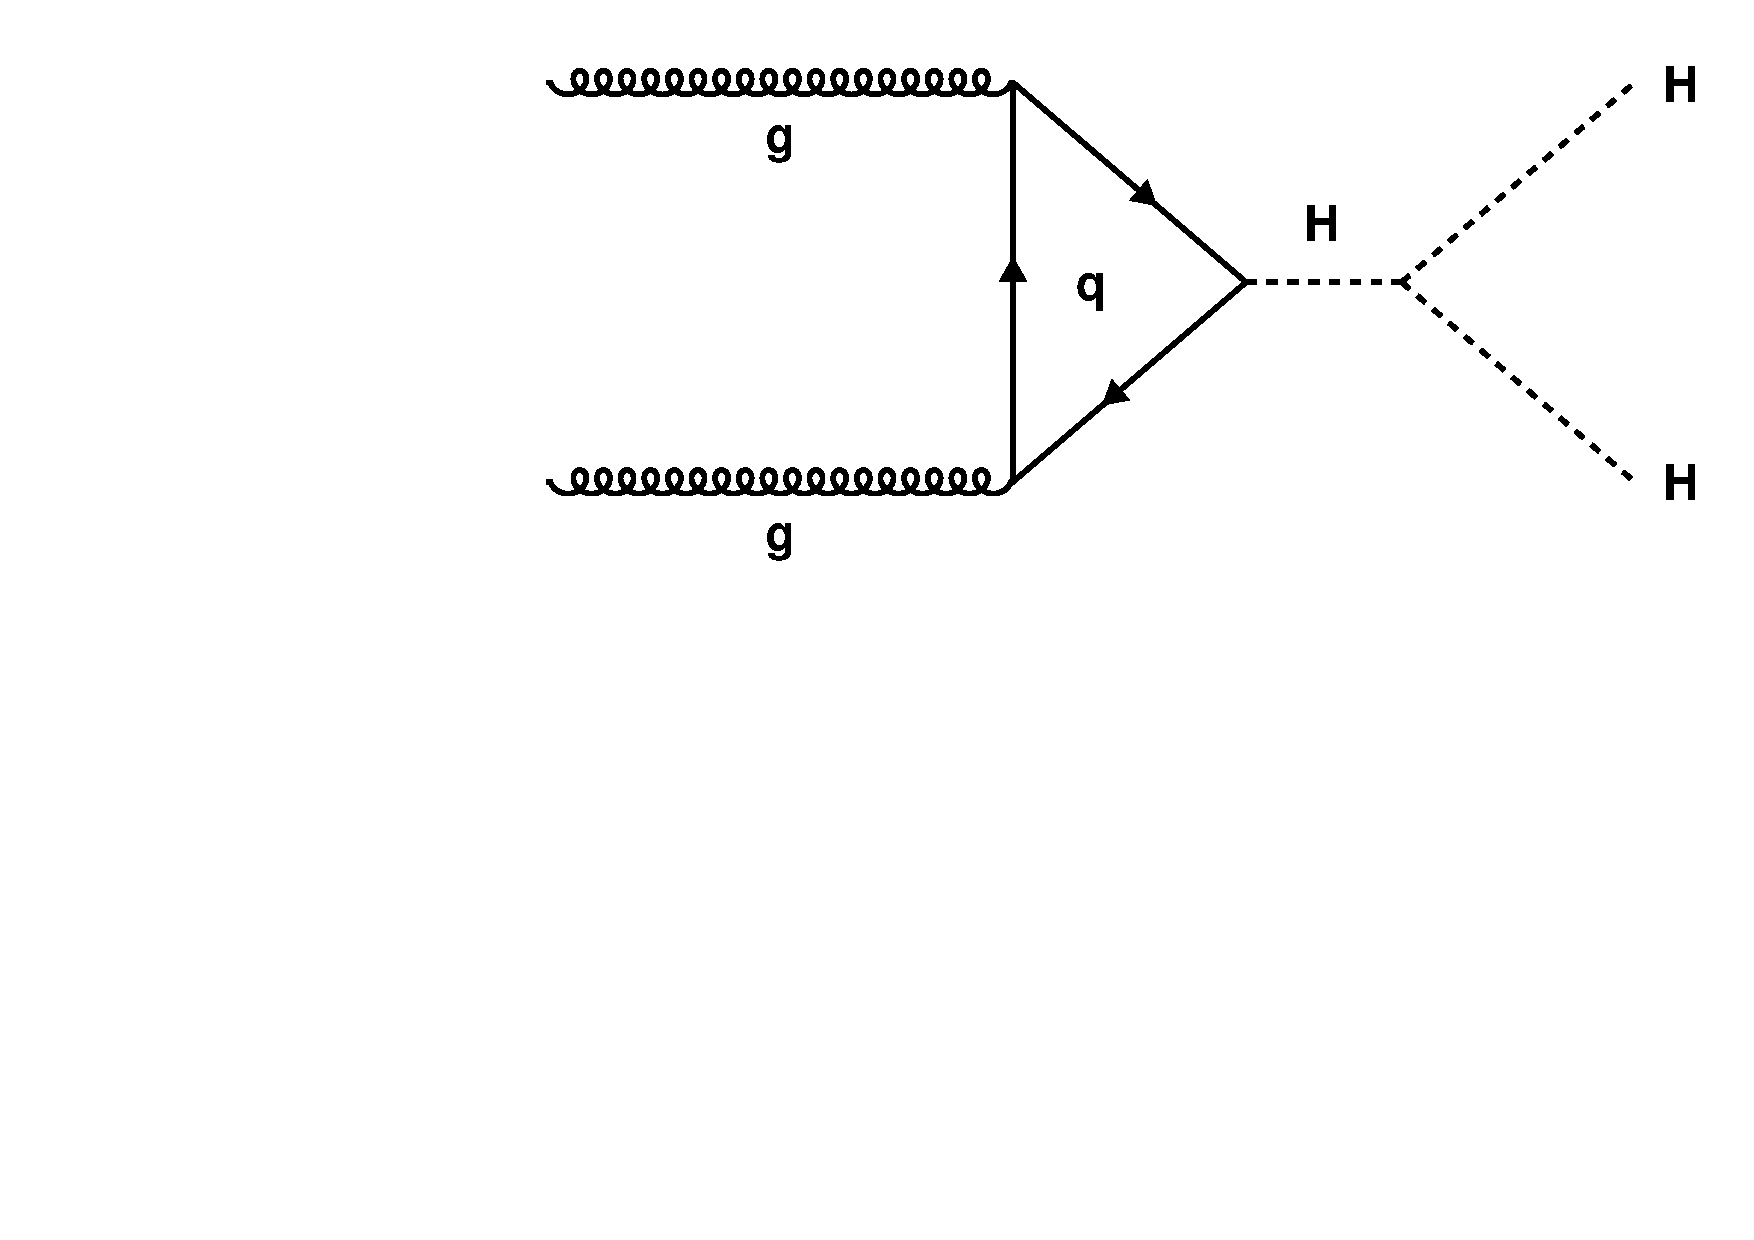
\includegraphics[width=0.40\textwidth]{figures/feynman_nonresonant_triangle.pdf} \hspace{\fill}
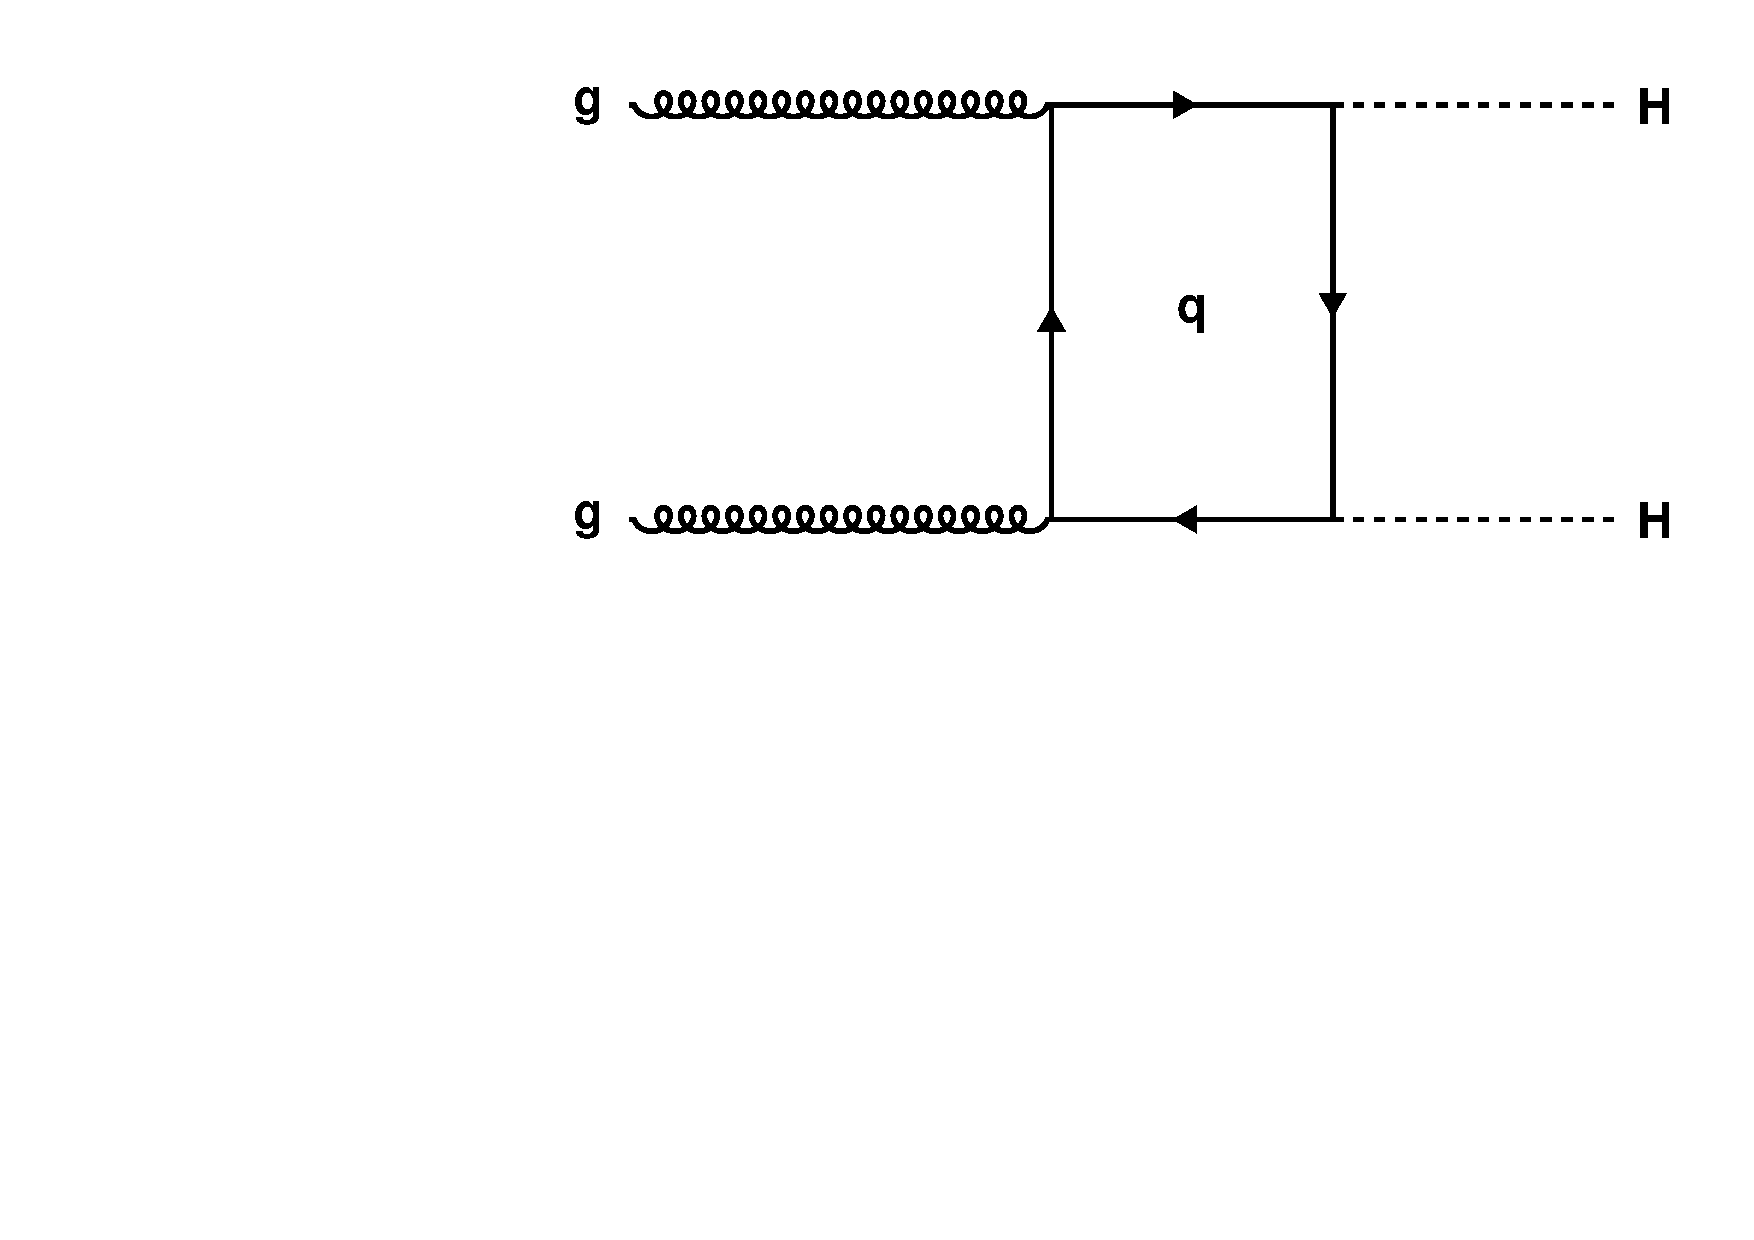
\includegraphics[width=0.40\textwidth]{figures/feynman_nonresonant_box.pdf} \hspace{\fill}
\caption{ LO Feynman diagrams for $\PHiggs\PHiggs$ production within the SM.}
\label{fig:FeynmanDiagrams_smHH}
\end{figure}

The rate for $\PHiggs\PHiggs$ production may be enhanced significantly in case as yet undiscovered heavy particles $\textrm{X}$ decay into pairs of $\PHiggs$ bosons.
Several models beyond the SM give rise to such decays, 
for example Higgs portal models~\cite{Englert:2011yb,No:2013wsa} and models involving warped extra dimensions~\cite{Randall:1999ee},
as well as two-Higgs-doublet models and models with composite Higgs bosons.
If the lifetime $t$ of these particles is sufficiently large compared to their mass $m_{\textrm{X}}$, $t \gtrsim 10^{-25}\textrm{~s}/m_{\textrm{X}}\textrm{~[100~GeV]}$, 
the distribution in the mass $m_{\PHiggs\PHiggs}$ of the $\PHiggs$ boson pair is expected to exhibit a narrow peak at $m_{\textrm{X}}$.

In this paper we present an algorithm for the reconstruction of the mass $m_{\PHiggs\PHiggs}$ of the $\PHiggs$ boson pair 
in events in which the $\PHiggs$ boson pair originates from the decay of a heavy particle $\textrm{X}$ and decays via $\PHiggs\PHiggs \to \Pgt^{+}\Pgt^{-}\Pgt^{+}\Pgt^{-}$,
with subsequent decay of the $\Pgt$ leptons into electrons, muons, or hadrons.
The decay of $\PHiggs$ boson pairs to four $\Pgt$ leptons ($\PHiggs\PHiggs \to \Pgt^{+}\Pgt^{-}\Pgt^{+}\Pgt^{-}$) has not been discussed in the literature so far.
This decay mode provides a small branching fraction, but also comparatively low backgrounds.
The algorithm achieves a resolution on $m_{\PHiggs\PHiggs}$ that varies between $3$ and $8\%$.
We expect that the reconstruction of $m_{\PHiggs\PHiggs}$ will significantly further improve the separation of the $\textrm{X} \to \PHiggs\PHiggs \to \Pgt^{+}\Pgt^{-}\Pgt^{+}\Pgt^{-}$ signal from backgrounds,
thereby increasing the sensitivity to either find evidence for the presence of such a signal in the LHC data or to set stringent exclusion limits.

The reconstruction of $m_{\PHiggs\PHiggs}$ in $\textrm{X} \to \PHiggs\PHiggs \to \Pgt^{+}\Pgt^{-}\Pgt^{+}\Pgt^{-}$ events is
based on the formalism for treating $\Pgt$ decays in the so-called matrix element (ME) method~\cite{Kondo:1988yd,Kondo:1991dw},
developed in Ref.~\cite{SVfitMEM}.
The algorithm presented in this paper does not employ the full ME formalism,
but uses a simplified likelihood function of arbitrary normalization.
The simplified approach is motivated by the studies performed in Ref.~\cite{SVfitMEM}, 
which found that the difference in mass resolution between the approximate likelihood treatment and the full ME formalism 
is small when reconstructing the mass of $\PHiggs$ bosons in events with single $\PHiggs$ bosons decaying via $\PHiggs \to \Pgt^{+}\Pgt^{-}$,
while the saving in computing time is significant.

The paper is organized as follows. 
The algorithm for reconstructing $m_{\PHiggs\PHiggs}$ is detailed in Section~\ref{sec:algorithm}.
In Section~\ref{sec:performance} we study the resolution achieved by our algorithm.
The paper concludes with a summary in Section~\ref{sec:summary}.
